\documentclass[a4paper]{article}
\usepackage{amsmath}
\usepackage{graphicx}
\usepackage{longtable}
\usepackage{makecell}
\usepackage[most]{tcolorbox}
\usepackage{listings}
\usepackage{csquotes}

\title{SDCND Traffic Sign Recognition}
\date{2019-04-09}
\author{Matthias Schinacher matthias.schinacher@googlemail.com}

\begin{document}

\maketitle
\tableofcontents
\newpage

\section{Intro}
The project is a homework assignment for Udacity's \textbf{Self Driving Car Nano Degree}.
The project is the third one called \textit{Traffic Sign Classifier}.
\\
The task is to train a neural network derived from or inspired by the LeNet-5 architecture
to identify 43 classes of German traffic signs within 32x32x3 pictures.
The goal accuracy is 93\%.

\subsection{Implementation}
As mandated the actual code implementation is within the Ipython notebook provided
with the project materials, that I adjusted/ expanded accordingly.

\section{Rubric criteria}
\subsection{General remarks}
Some of the criteria demand certain outputs by the notebook. Consequently the
respective documentation can be found in the solution run of the notebook
\enquote{Traffic\_Sign\_Classifier\_20190409\_04.html} together with the
files of the corresponding directory (I will refer to it as the \textbf{solution-html}).

\subsection{Criteria compliance}
\paragraph{Dataset Summary}
:\\
see output within \textit{solution-html}

\paragraph{Exploratory Visualization}
:\\
to get a better grip on the dataset I visualized the following:
\begin{itemize}
\item distribution of the frequencies of the different classes (say, the different signs) within the dataset and it's subsections (train, validate, test) as histograms
\item differences of the relative frequencies between the subsections as histograms
\item transformation of randomly chosen training images to other color spaces (HLS und LUV) and visualization of the various channels and some combination of channels
\end{itemize}

see the \textbf{actual output} within \textit{solution-html}.\\
The idea was, to better understand how uniform the distribution of classes would be
(I expected the training to be more difficult for non uniform distributions, since
classes with few examples are harder to learn), how similar the distributions were
(a test- dataset that is derived from an essentially different distribution compared to
validation and training will result in a lower test- accuracy) and if I could identify
maybe channels from color-spaces other than RGB and grayscale, that could help
in preprocessing.

\paragraph{Preprocessing}
:\\
The preprocessing finally used is a transform to grayscale and normalization.
\\
I did however experiment with the L- channel of the HLS space and with combinations
of that with the L and V channels from LUV; the resulting performance was not good :-).

\paragraph{Model Architecture}
:\\
I did experiment with various details (e.g. including bias for the conv. layers or not,
initialization of variables, ...) and number of layers, but not with the basic structure
of the model:
\begin{itemize}
\item the front layers are pairs of convolutional layers with ReLU activation and pooling layers
\item the rear layers are fully connected layers with optional ReLU and a dropout layer mixed in
\item convolutional layers use \enquote{valid padding} and only stride=1
\item pooling layers are max layers with \enquote{valid padding} and stride matching the kernel size
\end{itemize}

The detailed layer description of the \textit{solution}:
\small
\begin{enumerate}
\item convolutional layer with 3x3 kernel, 8 output channels, bias unit and ReLU activation; 32x32x1 $\rightarrow$ 30x30x8
\item pooling layer with 2x2 kernel; 30x30x8 $\rightarrow$ 15x15x8
\item convolutional layer with 6x6 kernel, 21 output channels, bias unit and ReLU activation; 15x15x8 $\rightarrow$ 10x10x21
\item pooling layer with 2x2 kernel; 10x10x21 $\rightarrow$ 5x5x21
\item flatten- layer; 5x5x21 $\rightarrow$ 525
\item fully connected layer with bias and ReLU; 525 $\rightarrow$ 180
\item dropout layer
\item fully connected layer without bias (and no ReLU); 180 $\rightarrow$ 43
\item softmax layer
\end{enumerate}
\normalsize

\textbf{Note:} with the preprocessing, the images fed to the NN were of technical dimension 32x32x1.

\paragraph{Model Training}
:\\
The actual training algorithm used is a simple one.\\
I used a standard Adam- optimizer with a cross-entropy- loss function and looped for a
predetermined number of steps over one optimizer-step using a random batch of training examples
of predefined size.\\
The program outputs the loss and accuracy of the current model \textbf{regarding
the complete training- set and the complete validation-set} frequently
to the screen/ browser and to a file; the actual model is also saved then, \textbf{if}
the validation-accuracy is the best yet.
\\
The random sampling of each batch is done using the complete training set.
I used this approach because of it's simplicity and to make the implementation easy,
but the approach does not guarantee that each training-example is used, and it
does not have the \textit{epoch}- concept.
\\
I would expect, such an approach has performance issues for very large datasets,
that do not fit in memory, since the whole dataset is potentially accessed for
each step.

\paragraph{Solution Approach}
:\\
The approach I used is mainly one of trial and error. I implemented a NN- model
derived as a mix from various different examples of a LeNet-5 like networks I researched
on the WWW. I ran the training and evaluation with different parameters and also
experimented a bit with the numbers and the sizes of layers.\\
The output to a textfile of the validation and training accuracy
once per \textit{validation-step} steps allowed for the evaluation of the
performance using a simple plot (using the gnuplot program).\\
Examples:\\
\begin{tabular}{ |c|c| }
  \hline
  \includegraphics[scale=0.3]{results_20190409111936.png} & \includegraphics[scale=0.3]{results_20190409112742.png} \\
  \hline
\end{tabular}

I experimented mostly with the number of steps to run, batch-size, drop-out-rate
and learning-rate (for the optimizer). E.g. I noticed, that the accuracy
approached the \textit{perfect score} of $1.0$ for the training-set, but would lack
for the validation-set; thus I presumed, the network was overfitting and adjusted
dropout-rate.

\paragraph{Test a Model on New Images}
:\\
I downloaded various traffic sign pictures from the WWW and used 4 of these pictures
plus 2 pictures I shot myself (for a total of 6) to test the model.
:\\
\small
\begin{tabular}{ |c|c|c| }
  \hline
  \includegraphics[scale=1.5]{tsign01.jpg} & 
\includegraphics[scale=1.5]{tsign08.jpg} & 
\includegraphics[scale=1.5]{tsign03.jpg} \\
  17: No entry & 13: Yield & 14: Stop \\
  \hline
  
\includegraphics[scale=1.5]{tsign06.jpg} & 
\includegraphics[scale=1.5]{tsign07.jpg} & 
\includegraphics[scale=1.5]{tsign09.jpg}\\
  5: Speed limit (80km/h) & 6: End of speed limit (80km/h) & 12: Priority road \\
  \hline
\end{tabular}
\normalsize

In my expectation these pictures should have been not to hard to classify, since
for all of them the lighting is quite good (not to dark) and can by readily recognized by a human.
Only for \enquote{5: Speed limit (80km/h)} and \enquote{12: Priority road} I was uncertain
whether additional objects directly connected to the signs (in fact fragments of other supplemental signs)
might interfere with the identification.
\\
To my surprise, the solution-model was only able to identify 4 of the 6 signs correctly
(see \textit{solution-html} for details) and obviously not because of additional adjacent sign-fragments.
The misidentified signs where:
\begin{itemize}
\item the Stop- sign \\
this was most puzzling, since it is such a distinct sign \textbf{and} the 5 top probabilities did not include the correct solution
\item the Speed limit (80km/h) sign \\
this seems to be a case of misidentified number, cause the highest probability assigned was also a speed limit sign,
and there where 2 more among the top 5, but none with the correct number
\end{itemize}

As said, for further details refer to \textit{solution-html}.

\section{Solution}

The solution used a \textit{learning-rate} of $0.0009$, a \textit{batch-size} of $711$
with a \textit{dropout-rate} of $0.5$ for $3500$ steps.\\
The resulting accuracy of the model after the last step was $0.941$ for the
\textbf{test-set} (! it worked), $0.954$ for the \textbf{validation-set}
and $1.0$ ($0.999971$) for the \textbf{training-set}.\\
\textit{(maybe the model is still overfitting the training set and we need to
introduce additional dropout layers or other techniques)}\\

$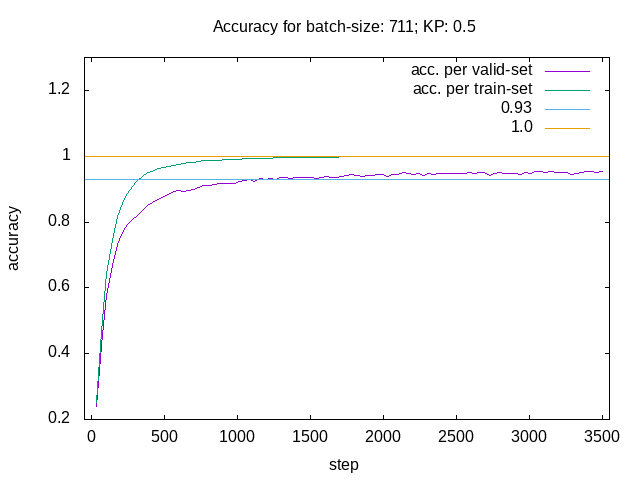
\includegraphics[scale=0.5]{results_20190409140717.png}$
\\
\textbf{\enquote{Solution files}}:\\
\tiny
\begin{itemize}
\item \texttt{Traffic\_Sign\_Classifier.ipynb}
\item \texttt{Traffic\_Sign\_Classifier\_20190409\_04.html}
\item files in directory \texttt{Traffic\_Sign\_Classifier\_20190409\_04\_files/}
\item \texttt{results\_20190409140717.txt}
\item \texttt{results\_20190409140717.png}
\end{itemize}
\normalsize

\end{document}
